%
%                       This is a basic LaTeX Template
%                       for the Informatics Research Review

\documentclass[a4paper,11pt]{article}
% Add local fullpage and head macros
\usepackage{head,fullpage}     
% Add graphicx package with pdf flag (must use pdflatex)
\usepackage[pdftex]{graphicx}  
% Better support for URLs
\usepackage{url}
% Date formating
\usepackage{datetime}
\usepackage{caption}
\usepackage{slashbox}
\usepackage[inline]{enumitem}
\usepackage{tikz}
\usepackage{amssymb}
\usepackage{graphics}
\def\checkmark{\tikz\fill[scale=0.4](0,.35) -- (.25,0) -- (1,.7) -- (.25,.15) -- cycle;}
\newcommand{\crossmark}{\scalebox{0.85}[1]{$\times$}}
\frenchspacing

\newdateformat{monthyeardate}{%
  \monthname[\THEMONTH] \THEYEAR}

\parindent=0pt          %  Switch off indent of paragraphs 
\parskip=5pt            %  Put 5pt between each paragraph  
\Urlmuskip=0mu plus 1mu %  Better line breaks for URLs


%                       This section generates a title page
%                       Edit only the following three lines
%                       providing your exam number, 
%                       the general field of study you are considering
%                       for your review, and name of IRR tutor

\newcommand{\examnumber}{B219992}
\newcommand{\field}{The Development of Emotion Recognition and Inference in Conversations}
\newcommand{\supervisor}{Shangmin Guo}

\begin{document}
\begin{minipage}[b]{110mm}
        {\Huge\bf School of Informatics
        \vspace*{17mm}}
\end{minipage}
\hfill
\begin{minipage}[t]{40mm}               
        \makebox[40mm]{
        
\includegraphics[width=40mm]{crest.png}}
\end{minipage}
\par\noindent
    % Centre Title, and name
\vspace*{2cm}
\begin{center}
        \Large\bf Informatics Research Review \\
        \Large\bf \field
\end{center}
\vspace*{1.5cm}
\begin{center}
        \bf \examnumber\\
        \monthyeardate\today
\end{center}
\vspace*{5mm}

%
%                       Insert your abstract HERE
%                       
\begin{abstract}
        %The abstract is a short concise outline of your 
        %project area, {\bf of no more than 100 words}.
        Emotion recognition in conversations is a growing area of research in the field of affective computing. Historically, various methods have been proposed for emotion inference in conversations including rule-based, machine learning-based, and deep learning-based approaches. In recent years, the use of pre-trained language models and transfer learning has been increasingly popular as a means of enhancing the capacities of emotion recognition in conversations. Another promising approach is the integration of common sense knowledge with emotion recognition models. Additionally, context and sentiment-aware graph networks have also been proposed as a method of improving the performance of these models. This literature review will contrast and compare these methods, discussing their limitations and advantages in order to provide a comprehensive overview of the current state of the field.
\end{abstract}

\vspace*{1cm}

\vspace*{3cm}
Date: \today

\vfill
{\bf Supervisor:} \supervisor
\newpage

%                                               Through page and setup 
%                                               fancy headings
\setcounter{page}{1}                            % Set page number to 1
\footruleheight{1pt}
\headruleheight{1pt}
\lfoot{\small School of Informatics}
\lhead{Informatics Research Review}
\rhead{- \thepage}
\cfoot{}
\rfoot{Date: \date{\today}}
%

\section{Introduction}

%This template can be used as a starting point for your \textbf{Informatics Research Review}. The template is based on \cite{template}.

%A literature review is an objective, critical summary of published research literature relevant to a topic under consideration for research. Its purpose is to create familiarity with current thinking and research on a particular topic, and may justify future research into a previously overlooked or understudied area.

%A typical literature review consists of the following components:

%\begin{enumerate}
    %\item A concise definition of a topic under consideration (this may be a descriptive or argumentative thesis, or proposal), as well as the scope of the related literature being investigated. (Example: If the topic under consideration is `women's wartime diaries', the scope of the review may be limited to published or unpublished works, works in English, works from a particular location, time period, or conflict, etc.)
    %\item The introduction should also note intentional exclusions. (Example: ``This review will not explore the diaries of adolescent girls'')
    %\item Another purpose of the introduction is to state the general findings of the review (what do most of the sources conclude), and comment on the availability of sources in the subject area.
%\end{enumerate}
The study of emotions is important as they shape our everyday experiences and activities. Research into emotions has numerous benefits, such as improving mental health diagnosis, enhancing customer satisfaction, revolutionising education and e-learning, better understanding user behavior on social media, making informed decisions in finance and investments, and improving urban design and architecture by analyzing human behavior. From the viewpoint of computer science, the investigation of emotions is carried out across various forms of media, including facial expressions, oral communication, and written text \cite{Li2018DeepFE,Drakopoulos2019EmotionRF,Marchal2019SurveyOA, 10.1145/3136755.3136801}. Traditionally, crafted characteristics, including identifying emotional keywords, utilising resources related to emotion vocabulary, and hashtags, were used to study emotions \cite{Strapparava2004WordNetAA, Wang2012HarnessingT}. However, with the advent of deep learning, researchers now have the ability to automatically learn features. 

In particular, the field of Natural Language Processing has seen a surge of attention directed towards emotion recognition (ERC) and emotion inference in conversations. This is partly due to the availability of a large volume of datasets, an increase in interest in dialogue-based technologies and casual argumentation, and the desire to create conversational agents that are better able to understand and respond to the emotions of those they interact with in a human-like manner \cite{Liu2021LifelongAC,Bowman2015ALA, Tu2021ExplorationME}. Challenges in these tasks go beyond the normal difficulties in understanding dialogue, such as identifying intent and considering context. It involves modelling the emotional dynamics between people and accounting for self and inter-speaker influences. Additionally, there are issues with the limited amount of annotated data, especially for multi-modal emotion recognition, and variability in annotations because emotions can be subjective to interpret \cite{Chen2017ASO,hazarika-etal-2018-icon,Hazarika2019ConversationalTL,Poria2020BeneathTT}.

In that aspect, there has been a lot of interesting research in these areas in recent years. Many scholars have used RNNs to analyse the context and sequence of utterances in conversations in order to recognise emotions. For instance, some researchers proposed using c-LSTM networks to record contexts \cite{poria-etal-2017-context}, while others such as \cite{Hazarika2018ConversationalMN} presented a memory network specifically designed for conversation which relied on GRUs. They established separate models for both the addresser and addressee, then utilised the desired utterance as a search item to probe the models to form a representation of the utterance. Hazarika et. al. utilised two GRUs to acquire the representation of the speaker's and the listener's utterance, then combined the outputs of these GRUs with another GRU to conduct inter-speaker modeling explicitly in \cite{hazarika-etal-2018-icon}. However both LSTMs and GRUs had certain pitfalls in this regard \cite{Bradbury2016QuasiRecurrentNN}. Several sophisticated techniques such as the DialogueRNN propose by Majumder et. al. tackled these issues by using GRUs to keep tabs on the party states, contextual information from preceding utterances and the emotions they entailed \cite{Majumder2018DialogueRNNAA}. Similarly, Ghosal et. al. put forward a new technique, using graph-neural networks that considered the relationships between and within speakers to capture context \cite{Ghosal2019DialogueGCNAG}. As for emotion inference, Hasegawa et. al. \cite{hasegawa-etal-2013-predicting} attempted to recognise and predict the emotional response of the listener in an online conversation. 

Despite their potential, there is still room for improvement in benchmark methods. The emergence of new areas such as transfer learning for sentiment analysis \cite{DavalFrerot2018EpitaAS}, incorporating external knowledge to make dialogue systems more intelligent \cite{Ma2020ASO}, and the use of pre-trained language models for dialogue-based tasks \cite{Bao2019PLATOPD} offer opportunities for further innovations and serves as the main theme of this review.

Specifically, some inquiries aim to evaluate if the recent techniques perform better in the following areas --
\begin{enumerate*}
    \item Resolving contextual ambiguities
    \item Operating with limited data availability
    \item Grasping the diversity and extents of emotions
    \item Identifying emotion shifts
    \item Comprehending the context, history, and intents of the speaker.
\end{enumerate*}

The rest of this paper is organised as follows. Section 2 addresses the research topics by examining four separate studies in subsections 2.1, 2.2, 2.3, and 2.4 for transfer learning, enhancing pre-trained language models, and common sense integration for emotion inference and recognition, respectively. Section 3 includes a short summary and conclusion.








\section{Literature Review}

%\begin{enumerate}
    %\item There are many ways to organize the evaluation of the sources. Chronological and thematic approaches are each useful examples.
    %\item Each work should be critically summarized and evaluated for its premise, methodology, and conclusion. It is as important to address inconsistencies, omissions, and errors, as it is to identify accuracy, depth, and relevance.
    %\item Use logical connections and transitions to connect sources.
%\end{enumerate}
\subsection{Transfer-Learning for Emotion Recognition}
\\
ERC is a complex endeavour that includes not only comprehending the intent and context of a conversation but also the capability to model the emotional modulation between speakers, taking into consideration the inter and self-speaker influences [3]. Furthermore, the task is hampered by the scarcity of annotated data, particularly in multimodal instances, and variances that arise as a result of the subjectivity of annotators in understanding emotions [4]. 

To tackle these challenges, Hazarika et. al. created the \textit{TL-ERC} paradigm, which employed sequential inductive transfer learning. The purpose was to use contextual affective information from a generative conversation modelling system to recognise emotions in natural conversations \cite{Hazarika2019ConversationalTL}. The novelty in their approach was to investigate and reason why generative models would see fit to gather insights about emotional dynamics. They used prior works to establish that emotional objectives and impacts worked as latent drivers in dialogues. The interconnectedness of numerous factors, such as the theme of the conversation, temperament of the speaker, their logical thought process, perspective and motivation, were responsible for altering their emotional state, eventually resulting in an utterance \cite{Weigand+1998+35+48, Poria2019EmotionRI}. The authors used example Fig \ref{emotional_dynamics} to demonstrate such inconspicuous emotional dynamics that organically craft conversations. In light of this, they speculated that since an ideal dialogue generator would need to decipher hidden emotions from the contextual settings of their historical utterances and characterise the trajectories underlying them, they might be able to depict implicit affective patterns throughout a conversation \cite{Shimizu2018PretrainingSC}. In order to transfer this knowledge into their intended discriminative task, namely ERC, they offered a strategy that employed transfer learning.

\begin{figure}[ht]
\centering
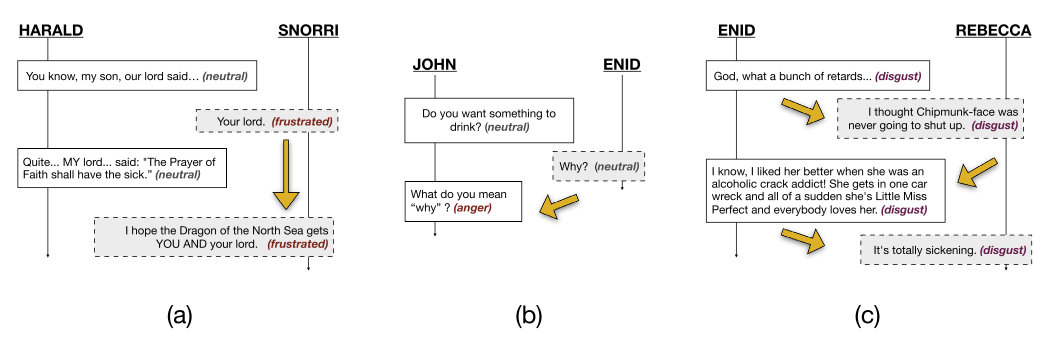
\includegraphics[width=0.9\textwidth]{Figures/Fig1-5.png}
\captionsetup{justification=centering}
\caption{Hazarika et. al. \cite{Hazarika2019ConversationalTL} -- Illustrations for the concepts of (a) \textit{emotional inertia} or self-influences in emotional states \cite{Koval2012ChangingED}, (b) \textit{emotional transitions} or \textit{shifts} due to external influences, and (c) \textit{mirroring} or topical agreement between speakers \cite{Navarretta2016MirroringFE}}
 \label{emotional_dynamics}
\end{figure}

The authors proposed to pre-train a hierarchical generative dialogue model on the \textit{source} task of conversation modelling as this unsupervised or self-supervised activity usually gained from a significant amount of data in the form of multi-turn dialogues. After pre-training, the model was fitted to the \textit{target} task of ERC by transferring the inter-sentence contextual parameters from the trained source model. To encode sentences, they used BERT \cite{Devlin2019BERTPO}, that is trained to meet concealed language modelling and next sentence prediction goals.

For the source task of generative conversation modelling, the authors used the Hierarchical Recurrent Encoder-Decoder (HRED), a traditional framework for seq2seq conversation answer generation that analyses conversations in a systematic order \cite{Serban2015BuildingED}, with three serial elements -- an encoder RNN for paired sentence and preceding context encoding, a context RNN for explicitly modelling the conversational context spanning utterances up until the current time-step $t$, and an auto-regressive decoder RNN for generating the response statement conditioned on the collective encoded context. Each conversation $C_i$ was considered as a collection of sequential utterances $[x_i,_1,...,x_i,_{n_i}]$. The HRED trained all conversations $C_i \in C$ in the dataset cumulatively by using the maximum likelihood estimate criterion $arg\,max_\theta = \sum log\,p_\theta(C_i)$. The authors used the original version of the HRED model architecture with single-layer components in order to keep the hypothesis simple and avoid the extra complexities of multi-layer RNNs and other novel encoding techniques provided by them. They modelled the encoder function of the sentence encoding RNN using a bi-directional Gated Recurrent Unit (GRU) \cite{Cho2014LearningPR} and used its uni-directional variant for the context encoder and decoder, while supplementing the decoder with a beam-decoding functionality as done by \cite{beam-decoding}.

 The infrastructural setup for the target task was similar to that of the source domain, as carried out by \cite{poria-etal-2017-context}, with the exception of the decoder being replaced by a discriminative mapping to the label space for classifying the emotion. The input to this model was a conversation $C$ with member utterances $[x_1,...,x_n]$ with each $x_i$ having an associated emotion label $y_i \in Y$. Hazarika et. al. utilised BERT \cite{Devlin2019BERTPO} to model utterances for the target task and expressed its parameters as $\theta^{BERT}$ (obtained from the source model - $\theta^{source}_{enc}$), only keeping the first four layers of the model to prevent parameter explosion. The hidden vectors of the $[CLS]$ token across were mean-pooled across the studied layers to obtain a sentence representation. They chose BERT as it outperformed the HRED sentence-encoder in terms of encoding power and inter-sentence level abstraction. The learned parameters of the GRU function of the context encoder in the source model were retained and transferred while an additional set of new weight and bias parameters were introduced for the dense layers in the target model, thereby leading to a final parametric representation $\theta^{source}_{cxt}$. The training of the classification layer was done using the cross-entropy loss and its output was the projection of the context RNN onto the label embedding space.

 Hazarika et. al. used the Cornell movie \cite{DanescuNiculescuMizil2011ChameleonsII} and Ubuntu dialog \cite{Lowe2015TheUD} corpora, two vast dyadic, bi-party conversational archetype datasets, to train their models for the conversation generation task. The dataset partitions were developed as recommended in \cite{Park2018AHL}. For the target task, they used the text mode of the small-sized dataset IEMOCAP, which consists of dyadic conversations between 10 speakers and emotion labels for \textit{anger, happiness, sadness, neutral, excitement}, and \textit{frustration}; the medium-sized chat-based dataset DailyDialog with emotion labels for \textit{anger, happiness, sadness, surprise, fear, disgust} and \textit{no\_emotion} \cite{Li2017DailyDialogAM}; and the regression-based dataset SEMAINE, a video-based corpus of human-agent emotional inflections \cite{5959155}. The dataset's emotional labels are \textit{valence, arousal, power} and \textit{expectation}, and the annotations were set up to be aligned with \cite{hazarika-etal-2018-icon}. 
 
 The DailyDialog dataset was very lopsided, in contrast to the well-balanced IEMOCAP dataset. The authors used the weighted F-score to evaluate these two datasets. However, the \textit{no\_emotion} class in the DailyDialog dataset had the most instances with 82.6\% and 81.3\% availability in the training and test sets, which made it difficult for them to objectively compare it to other classes and hence was not counted towards the F-score calculation. For the SEMAINE dataset, on the other hand, they employed the Pearson correlation coefficient $r$. They also defined an additional metric called the best epoch (BE) to convey information about the iteration at which the model performed optimally and where the validation loss was the smallest. The highest validation perplexity score was used to determine the pre-training weights for the source task \cite{Park2018AHL}. The authors employed the HRED-small model for the source task to prevent overfitting on the small-sized target datasets. The paper provides an in-depth explanation of the justification for this and other design options that were considered. For testing purposes, the authors created three versions of their \textit{TL-ERC} model with different parameter initialisation strategies. The first set of parameters used randomly sampled values for both the sentence and context encoders, the second used the pre-trained BERT model's sentence-encoding weights and randomly generated values for the context encoder, and the third used the pre-trained weights from BERT, and the training datasets, for the sentence and context encoders, respectively. They also contrasted their framework with a number of other cutting-edge benchmark models, including CNN \cite{Kim2014ConvolutionalNN}, Memnet \cite{Sukhbaatar2015EndToEndMN}, c-LSTM \cite{poria-etal-2017-context}, c-LSTM + Attn \cite{Poria2017MultilevelMA}, CMN \cite{Hazarika2018ConversationalMN}, and DialogueRNN \cite{Majumder2018DialogueRNNAA}.

Hazarika et al. examined the target data size, training time, and other design decisions in their model. First, they evaluated how well their model held up under the limited-data scenario. They did this by generating random subsets of their training data while keeping the label distributions static. When compared to models that had to undergo fresh training, they found that pre-trained models performed noticeably better in low-resource conditions. The third parametric variation of their model, which utilised pre-trained weights from both the BERT-based and source-context encoder, supported this (TL-based model) theory. The F-score for this version was the highest on the IEMOCAP and DailyDialog datasets. They also looked into the potential for bias in stochastic data splits. For this, they divided the IEMOCAP dataset by 10\% and 50\% and independently sampled 4 batches from it. Due to differences in their composition, each split produced divergent results, although the TL-based model consistently did better than the other variants in all cases. Additionally, they showed that the pre-trained model reached its best epoch much faster and converged on the validation loss more quickly. Another significant discovery in their work was the performance improvements BERT achieved over the HRED encoder. This showed that context-encoder performance depended on how well their sentence encoders performed.

The authors also aimed to determine if there was any correlation between the emotive content of the training data and the performance boost achieved by pre-training on them. To verify this, they set up an emotional profile by inspecting the vocabularies of the Ubuntu and Cornell datasets. Using the NRC emotion-lexicon \cite{Mohammad2013CROWDSOURCINGAW}, they assessed the affiliation of each token with an emotion. The authors concluded that the sources did not exhibit any differences in terms of results based on the F-scores obtained on the target datasets, when the pre-trained weights from the context encoder for each of the source datasets were used as the TL model's parameters and despite the Cornell dataset having a higher number of emotive tokens. The profiles were created by counting, lemmatising, and cross-referencing unique tokens in both datasets, according to the emotional overtones prompted by them. They also claimed that the identical performance gains in both situations could be explained by the fact that emotional profiles are more merely superficial, whereas response generation has emotion comprehension as an implicit function and is more innate in nature. The TL-ERC model outdid all comparison models, with a total F1 score of 58.8 on the IEMOCAP dataset, just behind DialogueRNN which had a score of 59.8 and used three layers between utterances, unlike TL-ERC's single layer.

Hazarika et. al. examined the reliability of their model and identified the difficulties faced during its training. They evaluated the impact of \textit{freezing} and \textit{fine-tuning} model weights during inductive transfer learning. The results indicated a decrease in performance from \textit{freezing}, as the model struggled with a large number of labels in the multi-class emotion recognition datasets and had a low recall on the scarce classes. They cautioned that trying to solve the issue by making adjustments or limiting the transferred parameters may result in an increased risk of overfitting. They also reasoned that \textit{fine-tuning} would present problems in terms of increased model complexity while trying to set an upper-bound on the number of transferable weights and finding a Goldilocks's zone for the optimal number of parameters in the target model that would yield performance gains. They also faced challenges with large fluctuations in standard error during the repeated training of their model using transferred weights, resulting in stability issues. Additionally, the authors attempted to enhance affective knowledge transfer by using a VHRED \cite{Serban2016AHL}, which is capable of encoding varying emotions for the same utterance rather than just a single label \cite{Provost2011AFF}. They also attempted to fine-tune the weights of the source model using conversation modelling in order to transfer it to the classification problem in the target model. However, the results indicated no substantial improvement in performance on any of the datasets. The authors also noted drawbacks in auto-regressive generative dialogue models, such as a lack of response diversity \cite{Li2015ADO} and consistency in emotions and themes \cite{Zhou2017EmotionalCM}. They saw the main weakness of HRED as its uni-directionality, which they believed was better addressed by transformer-based dialogue models that considered bi-directional contexts.






\subsection{Enhancing Pre-trained Language Models for Emotion Detection}
\\
Earlier, Hazarika et. al. \cite{Hazarika2019ConversationalTL} discussed the possibility of using transformers to capture context better and the need to find sentimental coherence between utterances, an area explored by the current study. Shen et. al. highlighted two key weaknesses of existing research in conversation modelling. They noted that many recent studies focused on encoding utterances as representations, which while systemically preserving the hierarchical and sequential organisation of dialogues, failed to facilitate pre-trained language models like BERT \cite{Devlin2019BERTPO} and XLNet \cite{Yang2019XLNetGA} from astutely capturing the direct dependencies between words in them. They also noted that these language models were handicapped by lengthy input sequences that frequently needed to be shortened, rendering them less advantageous due to the loss of information from far-off past utterances \cite{Ghosal2019DialogueGCNAG,Majumder2018DialogueRNNAA}. They reasoned that these models were not equipped to address more nuanced tasks like ERC, which encompass extensive chains of inter and intra speaker relationships \cite{Shen2020DialogXLAX}.

The primary objective of their work was to extend the capability of a pre-trained language model for the purpose of emotion recognition in dialogues. In order to combat the shortcomings presented by the aforementioned factors, they proposed a renewed model, DialogXL, a non-hierarchical network and adaptation of XLNet \cite{Yang2019XLNetGA}, for handling ERC in multi-turn and multi-party conversations. The development included two main ideas -- a) Replacing Transformer-XL's \cite{Dai2019TransformerXLAL} (from which XLNet was built) segment recurrence device with an \textit{utterance recurrence} mechanism to better capture historical context of up to a 1000 words. This enabled the model to better understand long-term dependencies, which are essential for tasks like ERC, that frequently deal with complete sentences and paragraphs. Additionally, this improvement also established a memory-efficient strategy for holding the hidden states of longer historical contexts into \textit{memory-banks} for future re-usability, by allowing for variable length sequences and releasing wasted padding memory blocks that were connected to fixed length sequences or \textit{segments}. b) Fleshing out the basic self-attention mechanism of the original transformer architecture with a \textit{dialogue-aware self-attention} component by infusing speaker roles and other relevant reception fields into it.

The embedding layer received an utterance prefixed with the \textit{[CLS]} token as input. The second tier of the DialogXL model was a transformer layer that included the previously stated \textit{utterance recurrence} and \textit{dialog aware self-attention} blocks. The memory unit in the utterance recurrence chamber concatenated and stacked the earlier utterances with the present one. To keep extraneous clutter away from the memory store, it contained an inherent mechanism that preserved just the hidden states of the utterance symbols along with the \textit{[CLS]} token and discarded the padding memory. The output from this block a new-updated memory. The attention segment contained four sub-units: a) Global self-attention, which took into account the context of all previous distant utterances; b) Local self-attention, with a flexible window size for receptive fields, where attention weights outside of the window were masked; c) Speaker self-attention; and d) Listener self-attention to model relationships between and within speakers, respectively. This unit did not require any additional embeddings or parameters. The outputs of the four sub-units were combined and then passed through a normalisation layer followed by a feed-forward network to generate the final output.

Shen et. al. evaluated their model on four datasets with emotions labels as follows -- IEMOCAP \cite{Busso2008IEMOCAPIE} :  \textit{neutral, happiness, sadness, anger, frustrated}, and \textit{excited}, DailyDialog \cite{Li2017DailyDialogAM} : \textit{neutral, happiness, surprise, sadness, anger, disgust}, and \textit{fear}, EmoryNLP \cite{Zahiri2017EmotionDO} : \textit{neutral, sad, mad, scared, powerful, peaceful}, and \textit{joyful} and MELD \cite{Poria2018MELDAM} : \textit{neutral, happiness, surprise, sadness, anger, disgust}, and \textit{fear}. As for the metrics, they chose the micro F1 score for the DialyDialog dataset, for reasons observed in the previous section on \cite{Hazarika2019ConversationalTL}. They made use of the weighted average F1 score for the remaining datasets. They compared their model's performance to the baseline approaches -- CMN \cite{Hazarika2018ConversationalMN}, DialogueRNN \cite{Majumder2018DialogueRNNAA}, TL-ERC \cite{Hazarika2019ConversationalTL}, DialogueGCN \cite{Ghosal2019DialogueGCNAG}, KET \cite{Zhong2019KnowledgeEnrichedTF} and HiGRU \cite{Jiao2019HiGRUHG}, BERT \cite{Devlin2019BERTPO} and XLNet \cite{Yang2019XLNetGA}.

Although DialogXL outperformed the leading-edge baseline models, it only slightly beat XLNet and BERT on short conversational datasets like DailyDialog, EmoryNLP, and MELD ($\approx$ 5-9 statements per conversation). Both XLNet and BERT were trained using the hyperparameters of DialogXL, with XLNet using segment recurrence and BERT using a combination of current and historical utterance representations. However, DialogXL outperformed all other models, including BERT and XLNet, on the long-utterance IEMOCAP dataset ($\approx$ 70 statements per conversation) with a weighted F1 score of 65.94. This showed that BERT and XLNet struggled to handle elongated contexts, while models like DialogueRNN and DialogueGCN, which encoded both speaker information and chronological contexts, were more effective in handling them. The authors evaluated three models to measure the waste of memory in terms of segment recurrence on the IEMOCAP dataset, which has long conversations per dialog. These models were: the original XLNet with segment recurrence, XLNet with utterance recurrence, and DialogXL. The latter two used utterance recurrence, leading to no padding memory waste. The experiment used a memory length capped at 1000 and an interval width of 100. The findings showed that the segment recurrence consistently caused a memory waste rate of 60\% or more. However, as the size increased, the rate gradually leveled off when the memory length surpassed 700, suggesting that increasing the memory length didn't necessarily have a significant benefit. Further investigations were conducted by the authors to assess the impact of each sub-unit of the \textit{dialog aware self-attention} module in DialogXL using the IEMOCAP and MELD datasets. The results reflected that the removal of the local self-attention had the largest effect on performance decline. This decrease was more pronounced on the IEMOCAP dataset, which consists of longer conversations. This demonstrated the significance of historical context neighbouring the current utterance. Another finding was that removing either listener or speaker self-attention or both had the second-highest impact on the model's performance. Both datasets showed similar results, highlighting the importance of inter and intra speaker dependencies. Finally, the authors found that the removal of global self-attention had the least effect on performance. They speculated that this could be due to either the global self-attention being less worthy or because the listener and speaker attentions caught some of the essential information from past utterances. Shen et. al. also experimented by replacing the listener and speaker self-attention mechanisms with a speaker role embedding vector \cite{Bao2019PLATOPD,Ham2020EndtoEndNP}. The F1 results from testing their DialogXL model on the DailyDialog and IEMOCAP datasets showed that this approach was not as effective as utilising the attention mechanisms directly. As a result, the authors suggest it as a potential addition to future models.

The researchers discovered that DialogXL's feature of grabbing details at the word-level from the historical contexts could sometimes backfire. The attention mechanism, centered around semantic relationships, had the potential to result in both accurate and inaccurate predictions. The negative scenario often occurred when a lot of importance was attached to past utterances. To illustrate their point, the researchers used two examples. In the first, the sentence \textit{``He's a fighter''} with the emotion label \textit{sad} was accurately predicted due to the preceding utterance \textit{``He's been sick for a while''} having a significant attention weight. However, the emotion label for the sentence \textit{``He was literally, literally the most talented guy''} was mistakenly predicted as \textit{happy} instead of \textit{sad}. This happened because the model placed too much emphasis on the previous utterance \textit{``And he's so talented''}, which on this occasion was used to express the speaker's regret for someone who had missed out on an opportunity. To achieve more reliable results in recognising emotions in dialogues, a more complete strategy was required instead of simply relying on attention mechanisms. Furthermore, the researchers noticed that a large portion (45\%) of the cases involving change in emotions between consecutive statements made by the same speaker resulted in errors, requiring additional thought.



\subsection{Incorporating Common Sense Knowledge for Emotion Deduction}
\\
Li et. al. investigated the concept of emotion inference, which sought to indicate how the contents of one subject's speech affected those of the other participants involved in a discussion. This work built on the prior theory of speaker interdependence and entailed comprehending emotions from the viewpoint of the addressee or listener. To accomplish this, they relied on identifying the addressee's function and simulating their emotional relationships with other speakers. This demanded the model to have causal reasoning abilities to meet this goal \cite{Li2021EnhancingEI}.  The authors contended that while deep learning had been explored heavily for emotion recognition, emotion inference and shift-detection in natural conversations remained understudied. The study by Hasewaga et. al. \cite{hasegawa-etal-2013-predicting}, which evoked listeners' feelings in  dialogues in uncomplicated online dialogue environments with no more than two conversation turns, was the only non-neural network method that most closely resembled their interests. The originality of Li et. al.'s approach was to build on this setting, scale it to multi-turn, multi-party conversations and give it resilience.

The stem for their study was rooted in achieving conversational intellect to solve real-world challenges like dialogue planning, interpretability and empathetic agents that are context-aware and can mimic human interactions. Li et. al. used a small yet fitting example to describe this phenomenon in practice. For instance, if Person Y's car broke down and Person X asked \textit{``Would you like a lift home?''}, a chat-bot would need to formulate its response using the emotion as a trigger to replicate human-like behaviour. In order to choose an appropriate response that is consistent with this emotion, it would first need to recognise that Person Y was sad about their broken-down car. It would then need to use its emotion inference component to determine whether Person Y's mood might change once Person X offered to drive them home, which most probably would reflect Person Y conveying a happy sentiment. Another possible outcome in this scenario is for Person Y to continue to feel depressed over their broken-down car and not exhibit a shift in their emotional state, despite being extended aid. As outlined in the previous cases, it's clear that the chat-bot might choose an unsuitable or even harmful response, without the ability of infer emotions.

The authors identified \textit{persistence} and \textit{contagiousness} \cite{10.1016/j.knosys.2019.105084, hazarika-etal-2018-icon} as the core elements of emotion inference. Of the two situations in the toy example above, the former involved contagiousness, where Person Y's state changed from sad to happy as a result of Person X's answer, and the latter involved persistence, where Person X's response had no effect on Person Y at all. The \textit{DialogInfer} framework developed by Li et. al. aimed to understand the emotional state of the person being spoken to in a conversation. It combined both a sequence-based and graph-based approach to gather information about both recent and past interactions and also included a built-in module to determine if the addressee's emotional state was primarily influenced by themselves or by others. Additionally, they proposed a technique to incorporate a particular kind of inferential knowledge into their model. They argued that while machines have difficulty understanding the causes and effects of events, humans can do so with ease. They integrated COMET \cite{bosselut-etal-2019-comet}, a conversation-related common-sense transformer model trained on inferential knowledge graphs to produce diverse and enriched knowledge, to get around this issue. ConceptNet \cite{Speer2016ConceptNet5A}, a semantic network with concept-level relational knowledge, and ATOMIC, an encyclopedia of 877k event-level textual descriptions of inferential knowledge and routine common sense reasoning \cite{10.1609/aaai.v33i01.33013027}, are the two knowledge bases on which COMET was trained. By using this special empirical information, the authors hoped to strengthen the ability of their model to infer emotions.

Li et. al. formulated a prediction problem to determine the addressee $p^a_m$’s emotional reaction $E_m^a$ to the utterance $U_m$, in a multi-turn, multi-party conversation. The inference was modelled on the entire conversation history --
$E_m^a \sim P(E_m^a |(U_1, p^w_1 ), (U_2, p^w_2 ), . . . , (U_m, p^w_m),\allowbreak p^a_m)$, where $(U_1,U_2,...,U_t,...,U_m)$ represented the complete list of utterances in a dialogue and $U_t$ was the utterance at time-stamp $t$ consisting of $N$ words. The notation $p$ with superscript $w$ was used to identify the role of a writer/speaker, while that with superscript $a$ pointed to the addressee/listener. In cases where the addressee was influenced by their own emotions, they assumed the same identity as the writer. 

The first step in the construction of the \textit{DialogInfer} architecture was to create a context-independent emotional representation $u_t$ for each utterance $U_t$. To this end, the authors used a CNN encoder with a 300-dimensional embedding layer of the pre-trained 840B GloVe vectors \cite{pennington-etal-2014-glove}. They utilised a range of filters with sizes of 3, 4, 5, and 50 to extract these features and encode all of the dataset's phrases with their emotional content as a 100-dimensional vector, which formed the encoder network's output layer. Additionally, they tuned the parameters of the pre-trained large-architecture RoBERTa-encoder to produce 1024-dimensional representations resembling those of the CNN counterpart, after initialising it using the values suggested in \cite{https://doi.org/10.48550/arxiv.1907.11692}.

The second stage involved creating an addressee-aware sequence-model. The intuition underlying this action was supported by the fact that utterances are sequential entities in the dialogue universe. Given that LSTMs have been successfully used for sequence classification tasks, the authors used them to model all conversations in their dataset \cite{Hochreiter1997LongSM}. For each time-step $t$, an LSTM-unit consisted of an input $x_t$, hidden-state $h_t$, cell-state $c_t$, input-gate $i_t$, forget-gate $f_t$ and output-gate $o_t$. The function of this component was to handle the gradual transmission of emotions over time. It was mathematically expressed as $(h_t,c_t) = LSTM(x_t, (h_{t-1},c_{t-1}))$. The importance of the cell-state $c^a_t$ and hidden-state $h^a_t$ was more officially highlighted by their responsibilities in recording and monitoring the internal and expressed emotional states of an addressee $p^a_m$. While the information at the internal emotional state $c^a_t$ was regulated by the input and forget gates $i_t$ and $f_t$, the data that culminated in the expressed emotional state $h^a_t$ was obtained by passing the signal from $c^a_t$ into the output-gate $o_t$. Two distinct types of specially designed LSTM cell layouts, each with its own set of parameters -- $LSTM_{store}$ and $\mathit{LSTM_{affect}}$, were used to control the process flow, which came in two kinds. According to the formal definition provided by Li et. al., the $LSTM_{store}$ unit would open its input-gate and store information into the internal state $c^a_t$ whenever the addressee spoke a historical utterance $u_t$ at time stamp $t$. The addressee and the writer had the same role in this case, and therefore $p^a_m = p^w_m$. This record was ideally required to examine how the addressee's past emotional states related to their future emotion, which carried the concept of \textit{persistence}. If, on the other hand, the addressee was influenced by another speaker's utterance $u_t$ at some time stp $t$ when $p^a_m \neq p^w_m$, the $LSTM_{store}$ opened its forget-gate to release the addressee's own previous state $c^a_{t-1}$ and altered the present state $c^a_t$ with this updated new knowledge. If the addressee was unaffected by the other participant's utterance, the $LSTM_{store}$ unit closed its input-gate and retained the addressee's prior state $c^a_t$. This exemplified the concept of \textit{contagiousness}. The final expressed emotional state $h^a_m$ was obtained by sending the last internal emotional state $c^a_m$ to an output-gate $o_m$. The $h^a_m$ was then loaded into an affine-layer with a ReLU activation function to produce the final emotional representation $es^a_m$ of the addressee $p^a_m$ at some time stamp $m$. The output representation was a 100-dimensional vector.

The third phase was to construct the graph-based addressee aware model, which recorded long-term historical information as opposed to the sequence model, which only assisted in recording short-term memories. Each graph node $g_t$ was instantiated with a linearly transformed utterance representation $u_t$, obtained from the CNN and RoBERTa-encoders. The node $g_t$ was then linked to each of its preceding sibling nodes $(g_{t-1},g_{t-2},....,g_{1})$ to gather all of the historical knowledge of the encoded utterances into it, based on the edge weights. There were a total of 100 nodes in the graph. The edges of the graph represented the dialogue states' relationships. Because the inference task required forecasting the addressee's present emotion, the nodes were only connected to their antecedents and future-state look-ahead operations were forbidden. The edge weights represented the degree of the interactions between nodes using a generalised attention function -- $ATT(g_m,g_t)$. Similar to the topology of the LSTM cells in the sequence model, two refined attention functions of the form $ATT_{persist}$ and $\mathit{ATT_{affect}}$ were adopted to differentiate between persistence and contagiousness. In cases where the addressee was the speaker of an utterance $u_t$ i.e., $p^a_m = p^w_m$, $ATT_{persist}$ was used to compute the edge weights between any two nodes $g_m$ and $g_t$ while $\mathit{ATT_{affect}}$ was used otherwise. The attention weight between nodes was calculated as a weighted combination of the two functions, and the node update for any node $g_m$ in the graph was executed as a linear sum of all the connected nodes and their previously computed attention coefficients. Finally, the addressee $p^a_m$'s emotion representation $eg^a_m$ was obtained by applying the ReLU activation function over the linear transform of the updated node values. Despite the fact that the network effectively captured and held long-term dependencies, the authors discovered that they paid greater attention to semantically connected nodes based on the attention value. To avoid completely excluding nodes that were not semantically connected and hence presumably less significant in predicting the addressee's emotion, they incorporated an unassuming contextual unidirectional LSTM to aggregate both types of information and integrated this into the graph model's emotion representation. This was formalised as -- $eg^a_m′ = eg^a_m + LSTM(u\leq m)$

The fourth and penultimate stage was commonsense knowledge integration. Li et. al. employed the COMET model to derive three categories of inferential knowledge -- $k^{oReact}_m$, $k^{oWant}_m$ and $k^\mathit{oEffect}_m$, from the input utterance $U_m$. According to the ATOMIC framework, each input phrase was formulated as a triplet $\{s, r, o\}$ where simply put, $s$ represented the phrase's subject or event description, $r$ represented the response or sentiment the event sparked in the participants, and $o$ represented the outcome or result of $r$. The paper provides a thorough explanation of the various facets of the ATOMIC knowledge base and is worth reading. The output phrases $k^{oReact}_m$, $k^{oWant}_m$ and $k^\mathit{oEffect}_m$ were then encapsulated to deduce the emotional reaction $ek^a_m$ of the addressee $p^a_m$ using a ReLU activation function and a linear transform layer.

As the fifth and last step, the emotion representations from the sequence-model $es^a_m$, graph-network $eg^a_m$ and knowledge-integration model $ek^a_m$ were concatenated to obtain the final emotion representation $e^a_m$ which was standardised as -- $e^a_m = \lambda_1 \cdot es^a_m + \lambda_2 \cdot eg^a_m + \lambda_3 \cdot ek^a_m$. $\lambda_1 = 1.0, \lambda_2 = 1.0$ and $\lambda_3 = 0.3$ were chosen and established as the optimal empirical hyper-parameter configuration by the authors. The final inferred emotion $E^a_m$ was obtained by passing $e^a_m$ through a linear classifier with the softmax activation function and $C$ output emotional categories. The authors postulated that by using ReLU to map all of the output vectors to a positive value space, rather than experimenting with various activation functions, they were able to prevent canceling positive and negative values in the parameterised summed representation for $e^a_m$.

Li et. al. evaluated their model on the IEMOCAP \cite{Busso2008IEMOCAPIE}, MELD \cite{Poria2018MELDAM} and EmoryNLP \cite{Zahiri2017EmotionDO} datasets and compared their results with several other state-of-the-art baseline neural-network based models such as the CNN \cite{Kim2014ConvolutionalNN} with GloVe embeddings, sc-LSTM \cite{poria-etal-2017-context}, DialogueRNN \cite{Majumder2018DialogueRNNAA}, DialogueGCN \cite{Ghosal2019DialogueGCNAG}, RoBERTa \cite{https://doi.org/10.48550/arxiv.1907.11692}, RoBERTa sc-LSTM, RoBERTa DialogueRNN, COMET \cite{bosselut-etal-2019-comet} and COSMIC \cite{Ghosal2020COSMICCK}. The also tried out different versions of their model including DialogInfer-S, DialogInfer-G, DialogInfer-G + sc-LSTM, DialogInfer-(S+G) and DialogInfer-(S+G)+K. The letters S, G, and K represented sequence-based awareness of the person being addressed, graph-based awareness of the person being addressed, and external knowledge of common sense, respectively. They conducted these tests both on the GloVe and RoBERTa versions. They utilised the weighted macro F1 score as their evaluation metric and the median scores from five iterations of each model variant was considered.

The authors followed Hasewaga et. al. \cite{hasegawa-etal-2013-predicting} to create training samples for the emotion inference task. They took the first $m$ exchanges as input and the label of the $(m+1)$th one as the prediction target. Only considering the participant information of the $(m+1)$th turn, they excluded the actual text of that turn from the input as the aim was to predict the emotional state of the addressee based on the first $m$ utterances without peeking into their impending reaction. For this reason, they adapted DialogueRNN, DialogueGCN, and COSMIC to suit the emotion inference endeavor by limiting their access to information about future utterances.

The \textit{DialogInfer-(S+G)+K} variant was found to be more effective than the baseline methods based on the weighted F1 scores of 61.03 and 65.20 for the GloVe and RoBERTa versions in the IEMOCAP dataset and 39.2 and 40.96 in the MELD dataset. The results of \textit{DialogInfer-S, DialogInfer-G}, and \textit{DialogInfer-(S+G)} also showed improved performance, demonstrating the advantage of taking into account both short and long term contexts. The higher scores for RoBERTa were likely due to its pre-training on vast amounts of unstructured text, making the features it extracted more valuable. The results for the EmoryNLP dataset were different, with the \textit{DialogInfer-(S+G)} and \textit{DialogInfer-S} models performing the best with F1 scores of 21.69 and 23.09 respectively, on both the GloVe and RoBERTa versions. The reason being that the EmoryNLP dataset has a fewer utterances from multiple speakers, and in such cases, incorporating longer historical contexts or external commonsense knowledge acted as a hindrance and corrupted the efficacy of original \textit{DialogInfer} model that included all three components. They also conducted experiments individually on the \textit{DialogInfer-S, DialogInfer-G, DialogInfer-G + sc-LSTM, DialogInfer-(S+G)} variants, without including the addressee-aware component, for all three datasets. The results, for both GloVe and RoBERTa, showed a decrease in F1 scores after excluding the addressee-aware module. This indicated that the segment effectively modelled the emotional impact and emotional contagion in conversations and could learn about the  emotion shifts experienced by the participants. To determine the usefulness of commonsense knowledge for emotion inference, the authors evaluated the performance of the COMET model that relied solely on commonsense information without the need for conversation utterances. The results of such knowledge bases (COMET and COSMIC) were compared to the baseline sentential-ERC models and it was observed that the models incorporating commonsense knowledge achieved equivalent results. This showed that the utilisation of external knowledge resources added significant value to the models and verified the proficiency of the integrated knowledge constituents. Li et. al. explored the impact of their addressee-aware module in the graph-based \textit{DialogInfer-G} model by illustrating the attention weights on the IEMOCAP dataset. The depictions showed that the module gave greater consideration to instances where the speaker and addressee were the same person. This was due to emotions being a persistent state, indicating a common human predisposition to be influenced by our own recent emotional experiences. The model was able to differentiate between different inputs and assign weights appropriately. Additionally, the graph-based model was intelligent enough to surpass time limitations when required and maintain them when the utterances were semantically linked, regardless of how far in the past they were. The authors also showed that including knowledge phrases from the external source COMET, which pertained to emotional reactions, desires, and effects (\textit{oReact, oWant} and \textit{oEffect}) of participants, provided a more focused view from the listener's perspective and enhanced the ability to infer their emotions. For instance, in one of the examples, Person A said \textit{``I'm sorry your husband cheated on you''}, for which the model was able to draw on its commonsense knowledge and infer that the listener (Person B) would feel \textit{sadness, pain}, or \textit{distress} and would feel the need to weep or end their marriage. This theoretical basis helped determine the listener's emotion, which in this case is \textit{melancholy}. Moreover, in many examples that observed emotion transmission trends, the authors noted the phenomenon of persistence in closely situated utterances (lower shift rates) while transitions between feelings of the same kind (e.g. happy and excited) were more pronounced (higher shift rates).

Although the \textit{DialogInfer} model was able to beat the baseline models' F1 scores by $\approx 3-4\%$ the authors encountered some deficiencies, especially with the class imbalance problem, as was  the case with the studies we have seen so far. For example, in the MELD dataset, emotion classes such as \textit{fear} and \textit{disgust} showed a lower representation. The authors argued that determining emotions was a challenging feat as individuals tend to see events subjectively and process them in different ways, and sometimes external knowledge sources can be unreliable to handle such large disparities.





\subsection{Emotion Recognition with Context and Sentiment Awareness}
\\
Tu et. al. attempted to solve a specific sort of issue connected with integrating common sense aspects for the purpose of ERC by building on earlier work. While previous studies dealt with addressee-aware models that sought to replicate contextual speaker dependencies infused with insights from common-sense knowledge bases, the authors discovered a gap in applying these relationships without accounting for the sentimental correctness between the target words and this information. They argued that it made no difference how the words were expressed when common-sense knowledge was inappropriately inserted into target utterances. Their inspiration originated from the actuality that remembered details could shift based on emotional influence. This idea, referred to as mood congruence effects \cite{Ekkekakis2013TheMO}, caused the authors to speculate that the depiction of common-sense in an ERC system may also be affected by feelings, which is a fluctuating process. Thus, a model that incorporated mood congruence effects not only considered the link between common-sense and contextual information, but also had the tendency to choose common-sense qualities that truly aligned with the sentiment expressed by the related words. Furthermore, to quantify the extent of this agreement, the utilisation of emotional intensity was also necessary. To that end, they developed \textit{Sentic GAT}, a framework that took both context and sentiment into account \cite{Tu2022ContextAS}. There were three primary parts to the framework and each of them are reviewed in the following paragraphs.

A dialogue transformer (DT) was used to record context-specific dependencies both within and between utterances. This network took advantage of the transformer's \cite{Vaswani2017AttentionIA} ability to model continuous interdependencies and semantic derivations \cite{Tang2018WhySA}. In order to represent historical contextual aspects of the target utterance instantaneously, the DT also used a hierarchical multi-head attention (HMAT) approach. To improve context approximations, the DT handled two separate vectors that performed context inference simultaneously throughout the training phase. While one of these encoded the context information, the other that did not. The two vectors were then given to a classifier, where a positive output of 1 signified a context-sensitive utterance and a value of 0 suggested a context-free utterance. To distinguish between these two types of samples, the authors investigated a contrastive-loss \cite{Gunel2020SupervisedCL, Khosla2020SupervisedCL} that separated samples with different labels while combining those with the same labels, allowing the distinction of context-free and context-sensitive vector representations.

The authors created a CSAGAT mechanism for incorporating sentimentally and conceptually congruent common-sense knowledge into the model. There were two aspects to this -- a) To preserve the sentiment consistency between the non-functional words in an utterance and their associated external concepts, and b) To understand the relationship between the external concepts and the context of the target utterance. The authors created a context-enriched representation of each utterance by modelling two types of weights. These weights were designed to reflect the role of context and sentiment awareness. More formally, they noted that the weight between tokens and concepts was influenced by both semantic similarity and the context-related information. They also suggested that the weight between tokens and concepts depended in part on the current sentiment of the speaker. This idea was based on the phenomenon of mood congruence. They also relied on describing the consistency of a sentiment, in terms of emotional intensity, which influenced the attention weights assigned to each relationship. The authors leveraged context awareness to incorporate external concepts into the model in a dynamic manner. The weight assigned to the external concepts was not only based on the assigned confidence score, but also adjusted based on the similarity between the concepts and the surrounding context information. As a result, when context changes were encountered, the same concepts were assigned different weights, leading to different representations of knowledge. The representation of the contextual utterances was determined by normalising and summing up their weighted n-gram representations. To arrive at the attention weights, the similarity between the concepts and the previously computed contextual-representations was evaluated while accounting for the confidence score. The weights of external concepts were adjusted depending on the sentiment of the current words and concepts. This was expressed by semantic awareness. To account for this, a threshold was established to decrease the weight of concepts that were inconsistent with the sentiment in the target utterance. This approach led to different knowledge representations for the same concepts when the associated words changed meanings. To quantify the degree of sentiment consistency, various models for describing emotions were employed. The attention weight after considering knowledge based on sentiment consistency was represented by $\varepsilon$ and the sentiment analysis techniques for multi-word and single-word concepts were borrowed from CoreNLP \cite{pennington-etal-2014-glove} and SenticNet \cite{Cambria2020SenticNet6E}, respectively. 
Additional functions to obtain the word and position embeddings were introduced. The calculation of emotional intensity was done using pre-built methods provided by emotional models like VAD \cite{Mehrabian1996PleasurearousaldominanceAG} and Hourglass \cite{Susanto2020TheHM}, which assessed various aspects of concepts in multiple dimensions. A parameterised combination of the context and sentiment weights thus resulted in a comprehensive and context-enriched representation of the utterance.

Tu et. al. evaluated their \textit{Sentic GAT} model on three datasets -- DailyDialog \cite{Li2017DailyDialogAM}, EmoryNLP \cite{Zahiri2017EmotionDO} and MELD \cite{Poria2018MELDAM}. For the metrics, they chose the micro F1 score for the DialyDialog dataset owing to the reasons seen previously in Hazarika et. al. \cite{Hazarika2019ConversationalTL} and \cite{Chatterjee2019UnderstandingEI}. For the other two datasets, they made use of the weighted average F1 score \cite{Majumder2018DialogueRNNAA}. They used ConceptNet -- a semantic graph in which words and sentences are linked by weighted edges (with weights representing confidence scores) and labels that indicate the edge-type \cite{Speer2016ConceptNet5A}, SenticNet --  a collection of 100,000 natural language ideas for semantics, emotion, and polarity. In particular, emotion alludes to the affective value of the four dimensions - \textit{introspection, temper, attitude}, and \textit{sensitivity} of the \cite{Susanto2020TheHM}. Semantics are the ideas that are most thematically connected to input concepts. Emotional polarity values lie between -1 and +1, where -1 is very negative and +1 is very positive \cite{Cambria2020SenticNet6E}, and NRC\_VAD -- an emotional lexicon of a set of words along with their associated VAD ratings for \textit{valence, arousal}, and \textit{dominance} which $\in$ [0,1] \cite{Mohammad2018ObtainingRH}, for commonsense knowledge integration.

They compared their results with several other baseline models such as c-LSTM \cite{poria-etal-2017-context}, DialogueRNN \cite{Majumder2018DialogueRNNAA}, DialogueGCN \cite{Ghosal2019DialogueGCNAG}, KET \cite{Zhong2019KnowledgeEnrichedTF}, RGAT \cite{Ishiwatari2020RelationawareGA}, SINN \cite{Feng2021SINNAS}, MVN \cite{Ma2021AMN} and PRE-CODE \cite{Jiao2020ExploitingUD}, as well as variants of their own \textit{Sentic GAT} model, such as \textit{CANet}, \textit{Sentic GAT\_VAD}, \textit{Sentic GAT\_Hourglass} and \textit{Sentic GAT\_Intensity}. When comparing the effectiveness of the aforementioned models on the three datasets, Tu et. al. found that KET (which employed a context-aware graph attention mechanism with common-sense knowledge) performed best among the baselines. However, they argued that KET only took emotional intensity into account, not sentiment consistency. On datasets like MELD and EmoryNLP that featured lengthy discussions, the \textit{CANet} model (the author's adaptation of \textit{Sentic GAT} without the sentiment-awareness component in CSAGAT), performed well; demonstrating the usefulness of their DT and context-aware graph attention method. Overall, across various test datasets, their proposed \textit{Sentic GAT} and its variations outperformed other models (with the exception of RGAT on the MELD dataset). They hypothesised that this was due to the fact that RGAT utilised BERT \cite{Devlin2019BERTPO} for utterance encoding, which according to them was more efficient than the GloVe embeddings that they used. To evaluate the emotional intensity of concepts, they included several emotion models and sentiment polarity to their \textit{Sentic GAT\_att2\_Intensity} variant, which then did better than RGAT on DailyDialog and EmoryNLP.

The authors also presented some additional analysis and shortcomings on various parts of their framework. They first discussed the context-awareness element which was meant to establish the relationship between external concepts and the current utterance and its surrounding statements. They found that by changing the context window size, the model's accuracy and F1 score showed an increase with the addition of more context information. However, after reaching a certain threshold, the model's performance started to deteriorate. They concluded that including more context enhanced the emotion recognition but too much context bore a negative impact. They also noted that the computational cost proportionally increased with larger context window sizes. They next examined the sentiment-awareness component to rate the impact of mood congruence on emotional recognition. Its purpose was to simulate the way humans select concepts to preserve the connection between sentiments and what they say. Results were analysed by changing a preset threshold value and observing how the accuracy and F1 scores changed. The graphs revealed that the peak F1 score varied between datasets, with a threshold of 0.3 in MELD, and 0.6 and 0.7 in DailyDialog and EmoryNLP, respectively. These numbers highlighted the importance of considering the degree of sentiment consistency with related knowledge, which is often complicated by the presence of sarcasm that in turn make deducing the attention weights and emotional intensity tough. The authors described this scenario by using the example of the happy word \textit{laugh} which in the MELD dataset, was used to represent a negative sentiment. They used their tabulated results on the F1 scores to substantiate that the HMAT did a fantastic job of collecting context information, far better than RNNs due to their shorter data flow circuits. However, they noticed that despite both EmoryNLP and MELD being long conversation datasets, HMAT fared poorly on EmoryNLP while doing well on MELD. As was previously seen, the authors implied that this would happen because some utterances in the dataset that properly predict the speakers' emotions without the need for, or with just a minimal usage of, context information. Therefore, providing too much background information for these sentences would be counterproductive or even detrimental. Based on the findings, it was also clear that contrastive loss had the greatest influence on the MELD dataset's outcomes and was essential for discriminating between context-free and context-sensitive utterances. The authors conducted a series of experiments to analyse the effect of different parts of \textit{Sentic GAT} on its performance. They found that the size of context utterances in CAGAT and the alignment of sentiments between concepts and related knowledge in SAGAT significantly impacted the network's ability to capture knowledge representation. Moreover, the relationship between and within historical utterances, which was measured by HMAT, influenced the precision of emotion detection. Results indicated that in both short and long conversations, CAGAT had the largest influence on the model's outcome, providing semantically enhanced features through concept embeddings and elevating the representation of knowledge with contextual information.

Tu et. al. pointed out that the F1 scores for the various emotions in their dataset varied based on the number of samples and the unbalanced distribution of emotions. The dataset, MELD, in particular, showed a low F1 score for the emotion of \textit{disgust}. The model was effective at identifying \textit{fear}, but struggled to distinguish between emotions. It frequently misclassified \textit{fear, sadness}, and \textit{anger} as \textit{disgust}. They reasoned that this may be due to the similarities between these emotions, as they are all fell under to the umbrella of negative emotions in SenticNet, with comparable degrees of emotional intensities in the Hourglass model, and low valence and high arousal in the VAD model. Hence emotion recognition becomes challenging while dealing with analogous emotions in class-imbalanced datasets.





\section{Summary \& Conclusion}

%\begin{enumerate}
    %\item The conclusion summarizes the key findings of the review in general terms. Notable commonalities between works, whether favourable or not, may be included here.
    %\item This section is the reviewer’s opportunity to justify a research proposal. Therefore, the idea should be clearly re-stated and supported according to the findings of the review.
%\end{enumerate}
To summarise, we evaluated four innovative methods that improve emotion recognition and inference in conversations and addressed most of the research questions raised at the start of the review. We evaluated them from the perspective of their methodologies, results, pros, cons and ablation studies. A common drawback among all models was that they did not perform well on short conversation datasets such as MELD and DailyDialog, possibly due to the them being overwhelmed by excess information. Table \ref{table:1} provides a summary of the datasets used and what remained to be explored in each approach. Other studies such as \cite{Gao2022EmotionRI,Ma2022EmotionRW,Fu2022ContextAK} also aimed to build upon the baseline methods. 
Another open question still exists. The authors mostly provided a general performance summary of their models, including a lack of examination of individual emotion classes in most cases and difficulty in distinguishing between similar emotions, as seen in Li et. al. \cite{Li2021EnhancingEI}. Future directions include using contrastive learning to distinguish closely related emotions, exploring the use of synthetic data, and studying emotion recognition, inference, and shift detection in low-resource languages through cross-lingual transfer learning and multilingual knowledge integration.

\begin{table}[ht]
\centering
\begin{tabular}{ |p{1.9cm}||p{2cm}|p{2.1cm}|p{2cm}|p{1.2cm}| p{2.01cm} |p{4cm}|}
 %\hline
 %\multicolumn{6}{|c|}{} \\
 \hline
 \textbf{Authors} & \textbf{IEMOCAP} & \textbf{DailyDialog} & \textbf{SEMAINE} & \textbf{MELD} & \textbf{EmoryNLP} & \textbf{Wasn't Explored} \\
 \hline
 Hazarika et. al.   & \checkmark    & \checkmark&  \checkmark & \crossmark & \crossmark & TL-ERC with hierarchical transformers \\
 \hline
 Shen et. al. &   \checkmark & \checkmark  & \crossmark & \checkmark & \checkmark & Emotion shifts. Speaker role embedding\\
 \hline
 Li et. al. & \checkmark & \crossmark & \crossmark & \checkmark & \checkmark & Addition of context including information about the setting, subject matter, and personalities of the individuals involved in the conversation. Improvement in the external knowledge used for inference. Issues with error analysis need to be tackled\\
 \hline
 Tu et. al. & \crossmark & \checkmark & \crossmark & \checkmark & \checkmark & Identify underlying ideas of common-sense knowledge through examination of sentiments or emotions at the word, sentence, and contextual levels. GCN to grasp the dependency between speakers, with the purpose of enhancing the accuracy of the model.\\
 \hline
\end{tabular}
\captionsetup{justification=centering}
\caption{Summary of the various datasets used by the discussed approaches and what remains to be explored by each of them}
\label{table:1}
\end{table}







%                Now build the reference list
\bibliographystyle{unsrt}   % The reference style
%                This is plain and unsorted, so in the order
%                they appear in the document.


\small
\bibliography{main}       % bib file(s).

\end{document}

